\documentclass[12pt, oneside]{article}
\usepackage[letterpaper, margin=1in]{geometry}
\usepackage[english]{babel}
\usepackage[utf8]{inputenc}
\usepackage{amsmath}
\usepackage{amsfonts}
\usepackage{amssymb}
\usepackage{tikz}
%\usepackage{tkz-fct}
\usepackage{pgfplots}
\pgfplotsset{width=10cm,compat=1.9}
\usepgfplotslibrary{statistics}
\usepackage{pgfplotstable}
%\usepackage{venndiagram}

\usepackage{fancyhdr}
\pagestyle{fancy}
\fancyhf{}
\rhead{\thepage \\Name: \hspace{1.5in}}
\lhead{BECA / Dr. Huson / 12.1 IB Math SL \\* 14 April 2018 \\*\textbf{Graphics examples
}}

\renewcommand{\headrulewidth}{0pt}

\title{pgfplots template}
\author{Chris Huson}
\date{April 2018}

\begin{document}
%\maketitle
\subsubsection*{\\ \textnormal{\textbackslash usepackage\{tikz\} \\ \textbackslash usepackage\{pgfplots\} \\
\textbackslash pgfplotsset\{width=10cm,compat=1.9\} \\
\textbackslash usepgfplotslibrary\{statistics\} \\
\textbackslash usepackage\{pgfplotstable\}
}}

\begin{enumerate}

\item Function in a box\\[5pt]
\begin{tikzpicture}
\begin{axis}
\addplot[]{exp(x)};
\end{axis}
\end{tikzpicture}\\


\item Function plot in color with legend, domain \& axes\\
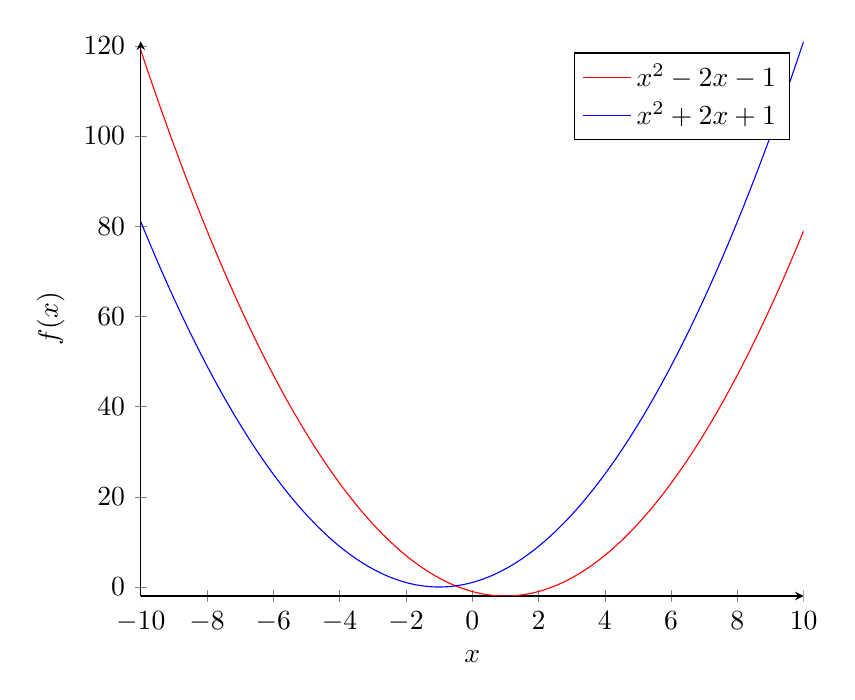
\begin{tikzpicture}
\begin{axis}[
    axis lines = left, %box, left, middle, center, right, none
    xlabel = $x$,
    ylabel = {$f(x)$},
    %mark = square,
]
\addplot [
    domain=-10:10,
    samples=100,
    color=red,
    ]
    {x^2 - 2*x - 1};
    \addlegendentry{$x^2 - 2x - 1$}
\addplot [
    domain=-10:10,
    samples=100,
    color=blue,
    ]
    {x^2 + 2*x + 1};
    \addlegendentry{$x^2 + 2x + 1$}
\end{axis}
\end{tikzpicture}\\

\item Scatter plots from data table\\
  \begin{tikzpicture}
    \begin{axis}[
        axis lines=middle,
        xmin=-10, xmax=10,
        ymin=-10, ymax=10,
        xtick=\empty, ytick=\empty
    ]
    \addplot [only marks] table {
    -10 -4
    -8  2
    -5  5
    -4  7
    -3  3
    0   6
    };
    \addplot [only marks, mark=o] table {
    -4  -5
    -2  -1
    -1  -4
    2   -3
    4   3
    6   -1
    };
    \addplot [domain=-10:10, samples=2, dashed] {1*x+3};
    \end{axis}
  \end{tikzpicture}

\item File data, scatter plot, titles\\
\begin{tikzpicture}
\begin{axis}[
    title={Data plot from file},
    axis lines = left,
    xlabel=$x$,
    ymin=0, ymax=21
    ]
\addplot[only marks, mark=*]
    table
    {sample-data.dat};
\addplot[color=red,
    domain=0:10
    ]
    {x+10};
\end{axis}
\end{tikzpicture}\\

Linear regression function (isn't quite working) (needs package pgfplotstable)\\
\begin{tikzpicture}
\begin{axis}[
    title={Linear Regression},
    axis lines = left,
    xlabel=$x$,
    ymin=0, ymax=21
]
\addplot[only marks, mark=*]
    table
    {sample-data.dat};
\addplot[color=red,
    domain=0:10,
    x=a,
    y={create col/linear regression={y=b}}
    ] %doesn't quite work. p27 in pgfplots docs
    table
    {sample-data-ab.dat};
\end{axis}
\end{tikzpicture}\\

\item Histogram (``ybar interval=1")\\[5pt]
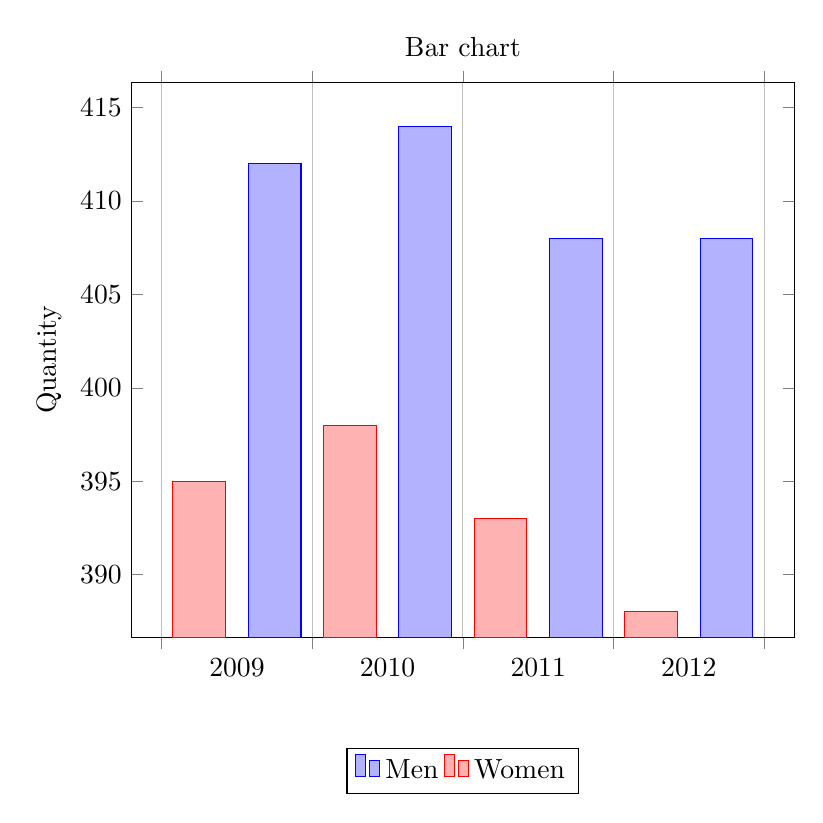
\begin{tikzpicture}
\begin{axis}[
    title={Bar chart},
    x tick label style={
		/pgf/number format/1000 sep=},
	ylabel=Quantity,
	enlargelimits=0.05,
	legend style={at={(0.5,-0.2)},
	anchor=north,legend columns=-1},
	ybar interval=.7,
]
\addplot
	coordinates {(2012,408) (2011,408)
		 (2010,414) (2009,412) (2008,415)};
\addplot
	coordinates {(2012,388) (2011,393)
		(2010,398) (2009,395) (2008,398)};
\legend{Men,Women}
\end{axis}
\end{tikzpicture}

\item Fancy scientific example\\
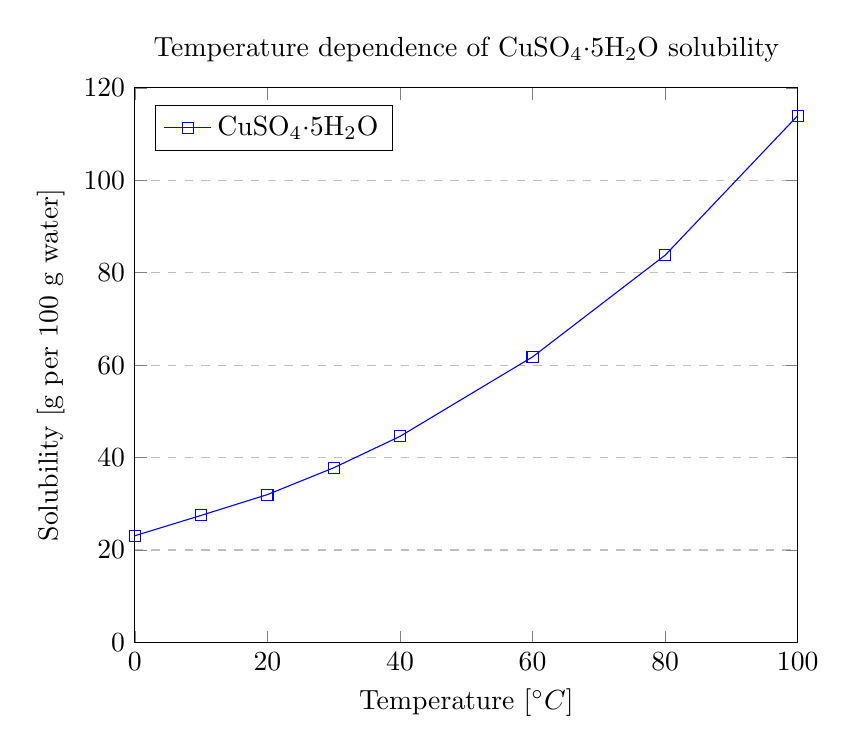
\begin{tikzpicture}
\begin{axis}[
    title={Temperature dependence of CuSO$_4\cdot$5H$_2$O solubility},
    xlabel={Temperature [$^{\circ}C$]},
    ylabel={Solubility [g per 100 g water]},
    xmin=0, xmax=100,
    ymin=0, ymax=120,
    xtick={0,20,40,60,80,100},
    ytick={0,20,40,60,80,100,120},
    legend pos=north west,
    ymajorgrids=true,
    grid style=dashed,
]
\addplot[
    color=blue,
    mark=square,
    ]
    coordinates {
    (0,23.1)(10,27.5)(20,32)(30,37.8)(40,44.6)(60,61.8)(80,83.8)(100,114)
    };
    \legend{CuSO$_4\cdot$5H$_2$O}
\end{axis}
\end{tikzpicture}

\item Box plot, various algorithm calculations from data file are possible (not quite working)\\
\begin{tikzpicture}
\begin{axis}[
    title={Box \& whisker plot, ``boxplot prepared"},
    axis lines=left,
    y=1cm,
    ytick={1,2,3},
    yticklabels={Group A, Group B, Group C},
	enlargelimits=0.05,
    ]
    \addplot+ [boxplot]
    table {sample-data-ab.dat};
   \addplot+ [
    boxplot prepared={draw position=0, %?
        lower whisker=6, lower quartile=9,
        median=10,
        upper quartile=11.8, upper whisker=13,
        },
    ] coordinates {(0,4)};% outliers here, or blank
    \addplot+ [
        boxplot prepared={
            lower whisker=5,
            lower quartile=7,
            median=8.5,
            upper quartile=9.5,
            upper whisker=10,
        },
    ] table [row sep=\\,y index=0] {
        data\\ 1\\ 3\\
    };
\end{axis}
\end{tikzpicture}

%\vspace{0.5 cm}
\subsubsection*{Expected value given table (fair)}
\item Given the following probability distribution, with $E(x)=2.5$ \\
\begin{tabular}{|c|r|r|r|r|}
\hline
$x$ & 0 & 1 & 2 & 4 \\
\hline
P(x) & p & 0.3 & 0.1 & q  \\
\hline
\end{tabular}
\begin{enumerate}
    \item Find the value of \hskip 25pt $p$
    \item Find the value of $q$
\end{enumerate}


\end{enumerate}
\end{document}
